\subsubsection{Filtro Sallen Key}

La tabla \ref{tab:filtro-sallen-key-ganancia-frecuencia} muestra los resultados obtenidos para el filtro Sallen Key, donde se puede observar la respuesta en frecuencia del filtro.

\begin{table}[h!]
    \centering
    \begin{tabular}{|c|c|c|c|c|c|c|c|c|c|}
        \hline
        $V_i$ (V) & $\Delta V_i$ (V) & $V_o$ (V) & $\Delta V_o$ (V) & T (ms) & $\Delta$T (ms) & Ganancia & $\Delta$Ganancia & f (Hz) & $\Delta$f (Hz) \\
        \hline
        1.0 & 0.1 & 2.0 & 0.1 & 1.0 & 0.04 & 2.000 & 0.224 & 1000.0 & 40.0 \\
        1.0 & 0.1 & 2.0 & 0.1 & 0.68 & 0.04 & 2.000 & 0.224 & 1470.6 & 86.5 \\
        1.0 & 0.1 & 1.4 & 0.4 & 0.33 & 0.01 & 1.400 & 0.424 & 3030.3 & 91.8 \\
        1.0 & 0.1 & 0.08 & 0.004 & 0.064 & 0.002 & 0.080 & 0.009 & 15625.0 & 488.3 \\
        1.0 & 0.1 & 0.18 & 0.01 & 0.1 & 0.004 & 0.180 & 0.021 & 10000.0 & 400.0 \\
        1.0 & 0.1 & 0.68 & 0.02 & 0.32 & 0.01 & 0.680 & 0.071 & 3125.0 & 97.7 \\
        1.0 & 0.1 & 1.6 & 0.04 & 0.36 & 0.01 & 1.600 & 0.165 & 2777.8 & 77.2 \\
        1.0 & 0.1 & 2.0 & 0.1 & 10.0 & 0.4 & 2.000 & 0.224 & 100.0 & 4.0 \\
        \hline
    \end{tabular}
    \caption{Mediciones de ganancia y frecuencia del filtro Sallen Key.}
    \label{tab:filtro-sallen-key-ganancia-frecuencia}
\end{table}



La figura \ref{fig:filtro-sallen-key} muestra el filtrado de la tercera armonica a la señal de entrada cuadrada.


\begin{figure}[h!]
    \centering
    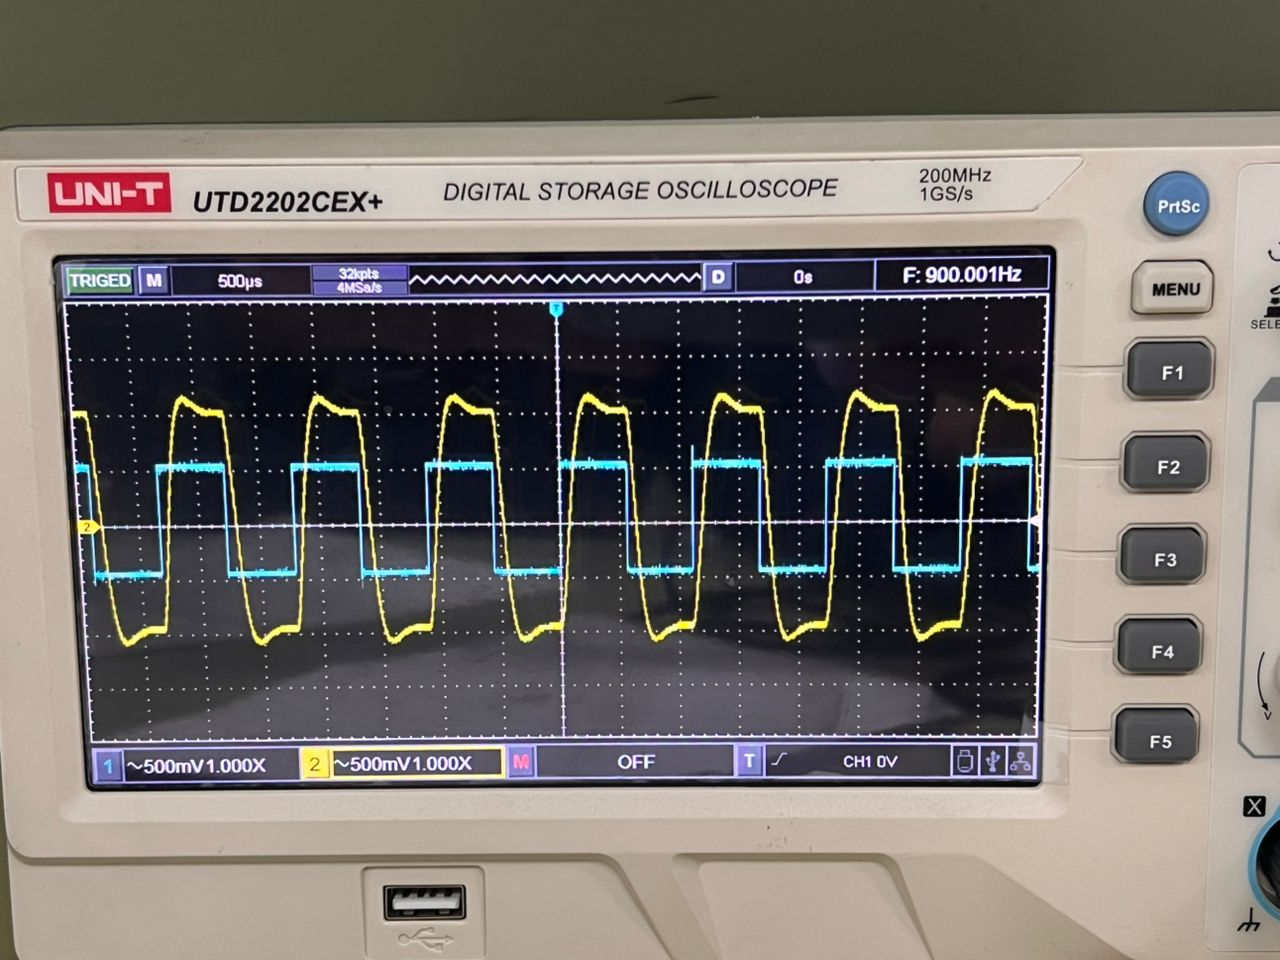
\includegraphics[width=0.5\textwidth]{resultados/filtro-sallen-key.jpg}
    \caption{Filtro Sallen Key: filtrado de tercera armonica.}
    \label{fig:filtro-sallen-key}
\end{figure}



\subsubsection{Filtro de realimentacion multiple}

La tabla \ref{tab:filtro-realimentacion-multiple-ganancia-frecuencia} muestra los resultados obtenidos para el filtro de realimentación múltiple, donde se puede observar la respuesta en frecuencia del filtro.

\begin{table}[h!]
    \centering
    \begin{tabular}{|c|c|c|c|c|c|c|c|c|c|}
        \hline
        $V_i$ (V) & $\Delta V_i$ (V) & $V_o$ (V) & $\Delta V_o$ (V) & T (ms) & $\Delta$T (ms) & Ganancia & $\Delta$Ganancia & f (Hz) & $\Delta$f (Hz) \\
        \hline
        1.0 & 0.1 & 2.2 & 0.2 & 10.0 & 0.4 & 2.200 & 0.297 & 100.0 & 4.0 \\
        1.0 & 0.1 & 1.5 & 0.1 & 0.27 & 0.01 & 1.500 & 0.180 & 3703.7 & 137.2 \\
        1.0 & 0.1 & 2.2 & 0.1 & 1.0 & 0.04 & 2.200 & 0.242 & 1000.0 & 40.0 \\
        1.0 & 0.1 & 1.5 & 0.1 & 0.68 & 0.04 & 1.500 & 0.180 & 1470.6 & 86.5 \\
        1.0 & 0.1 & 1.7 & 0.1 & 0.30 & 0.04 & 1.700 & 0.197 & 3333.3 & 444.4 \\
        1.0 & 0.1 & 1.3 & 0.1 & 0.25 & 0.01 & 1.300 & 0.164 & 4000.0 & 160.0 \\
        1.0 & 0.1 & 1.2 & 0.1 & 0.12 & 0.01 & 1.200 & 0.156 & 8333.3 & 694.4 \\
        1.0 & 0.1 & 0.1 & 0.01 & 0.064 & 0.002 & 0.100 & 0.014 & 15625.0 & 488.3 \\
        \hline
    \end{tabular}
    \caption{Mediciones de ganancia y frecuencia del filtro de realimentación múltiple.}
    \label{tab:filtro-realimentacion-multiple-ganancia-frecuencia}
\end{table}


\begin{figure}[ht]
    \centering
    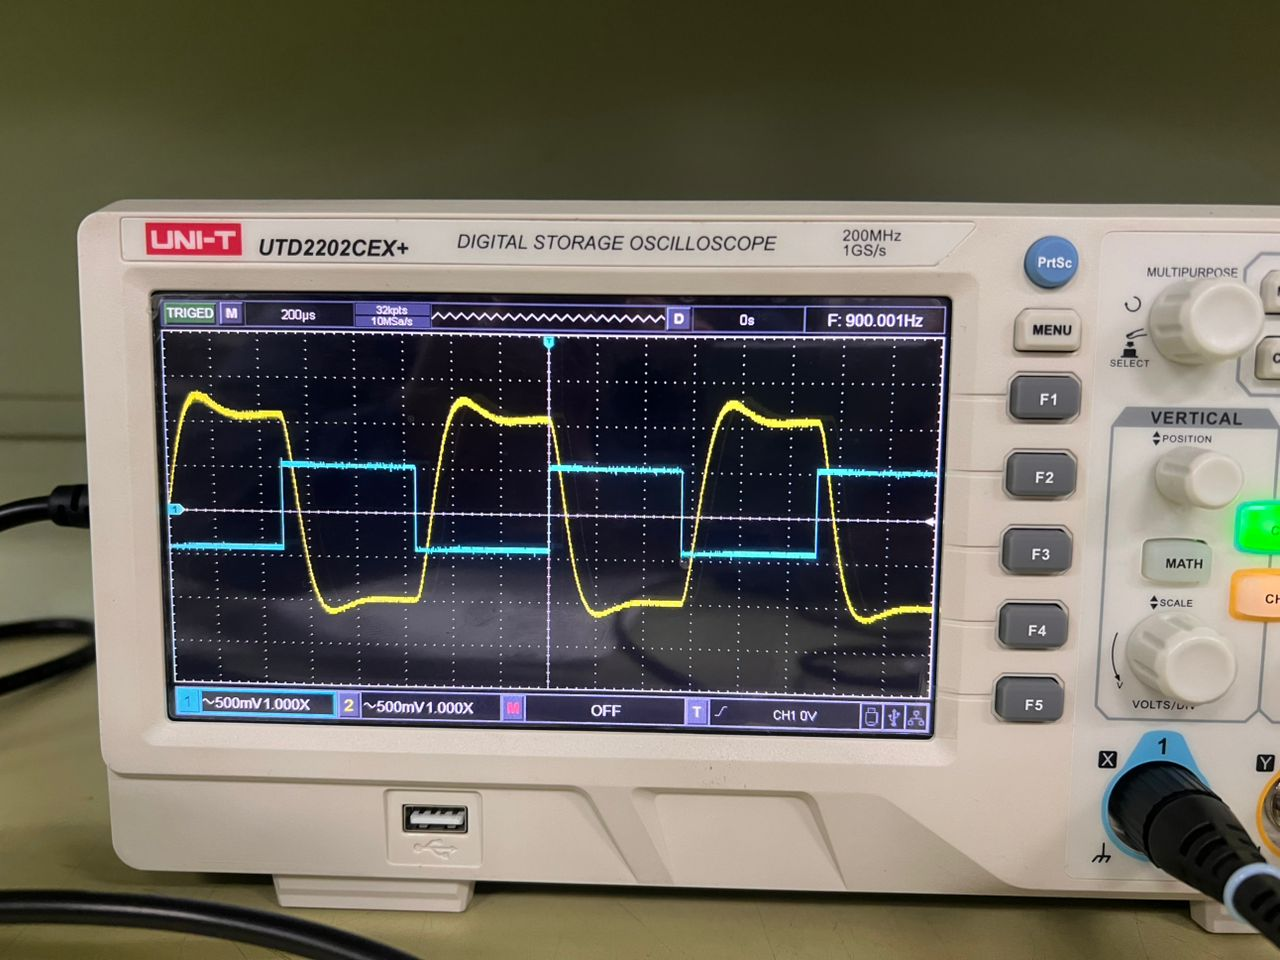
\includegraphics[width=0.5\textwidth]{resultados/filtro-realimentacion-multiple.jpg}
    \caption{Filtro de realimentación múltiple: filtrado de tercera armonica.}
    \label{fig:filtro-realimentacion-multiple-tercera-armonica}
\end{figure}